\documentclass[twoside]{book}

% Packages required by doxygen
\usepackage{calc}
\usepackage{doxygen}
\usepackage{graphicx}
\usepackage[utf8]{inputenc}
\usepackage{makeidx}
\usepackage{multicol}
\usepackage{multirow}
\usepackage{textcomp}
\usepackage[table]{xcolor}

% Font selection
\usepackage[T1]{fontenc}
\usepackage{mathptmx}
\usepackage[scaled=.90]{helvet}
\usepackage{courier}
\usepackage{amssymb}
\usepackage{sectsty}
\renewcommand{\familydefault}{\sfdefault}
\allsectionsfont{%
  \fontseries{bc}\selectfont%
  \color{darkgray}%
}
\renewcommand{\DoxyLabelFont}{%
  \fontseries{bc}\selectfont%
  \color{darkgray}%
}

% Page & text layout
\usepackage{geometry}
\geometry{%
  a4paper,%
  top=2.5cm,%
  bottom=2.5cm,%
  left=2.5cm,%
  right=2.5cm%
}
\tolerance=750
\hfuzz=15pt
\hbadness=750
\setlength{\emergencystretch}{15pt}
\setlength{\parindent}{0cm}
\setlength{\parskip}{0.2cm}
\makeatletter
\renewcommand{\paragraph}{%
  \@startsection{paragraph}{4}{0ex}{-1.0ex}{1.0ex}{%
    \normalfont\normalsize\bfseries\SS@parafont%
  }%
}
\renewcommand{\subparagraph}{%
  \@startsection{subparagraph}{5}{0ex}{-1.0ex}{1.0ex}{%
    \normalfont\normalsize\bfseries\SS@subparafont%
  }%
}
\makeatother

% Headers & footers
\usepackage{fancyhdr}
\pagestyle{fancyplain}
\fancyhead[LE]{\fancyplain{}{\bfseries\thepage}}
\fancyhead[CE]{\fancyplain{}{}}
\fancyhead[RE]{\fancyplain{}{\bfseries\leftmark}}
\fancyhead[LO]{\fancyplain{}{\bfseries\rightmark}}
\fancyhead[CO]{\fancyplain{}{}}
\fancyhead[RO]{\fancyplain{}{\bfseries\thepage}}
\fancyfoot[LE]{\fancyplain{}{}}
\fancyfoot[CE]{\fancyplain{}{}}
\fancyfoot[RE]{\fancyplain{}{\bfseries\scriptsize Generated on Wed Oct 30 2013 12\-:08\-:14 for qt-\/project1 by Doxygen }}
\fancyfoot[LO]{\fancyplain{}{\bfseries\scriptsize Generated on Wed Oct 30 2013 12\-:08\-:14 for qt-\/project1 by Doxygen }}
\fancyfoot[CO]{\fancyplain{}{}}
\fancyfoot[RO]{\fancyplain{}{}}
\renewcommand{\footrulewidth}{0.4pt}
\renewcommand{\chaptermark}[1]{%
  \markboth{#1}{}%
}
\renewcommand{\sectionmark}[1]{%
  \markright{\thesection\ #1}%
}

% Indices & bibliography
\usepackage{natbib}
\usepackage[titles]{tocloft}
\setcounter{tocdepth}{3}
\setcounter{secnumdepth}{5}
\makeindex

% Hyperlinks (required, but should be loaded last)
\usepackage{ifpdf}
\ifpdf
  \usepackage[pdftex,pagebackref=true]{hyperref}
\else
  \usepackage[ps2pdf,pagebackref=true]{hyperref}
\fi
\hypersetup{%
  colorlinks=true,%
  linkcolor=blue,%
  citecolor=blue,%
  unicode%
}

% Custom commands
\newcommand{\clearemptydoublepage}{%
  \newpage{\pagestyle{empty}\cleardoublepage}%
}


%===== C O N T E N T S =====

\begin{document}

% Titlepage & ToC
\hypersetup{pageanchor=false}
\pagenumbering{roman}
\begin{titlepage}
\vspace*{7cm}
\begin{center}%
{\Large qt-\/project1 }\\
\vspace*{1cm}
{\large Generated by Doxygen 1.8.5}\\
\vspace*{0.5cm}
{\small Wed Oct 30 2013 12:08:14}\\
\end{center}
\end{titlepage}
\clearemptydoublepage
\tableofcontents
\clearemptydoublepage
\pagenumbering{arabic}
\hypersetup{pageanchor=true}

%--- Begin generated contents ---
\chapter{Namespace Index}
\section{Namespace List}
Here is a list of all namespaces with brief descriptions\-:\begin{DoxyCompactList}
\item\contentsline{section}{\hyperlink{namespace_ui}{Ui} }{\pageref{namespace_ui}}{}
\end{DoxyCompactList}

\chapter{Hierarchical Index}
\section{Class Hierarchy}
This inheritance list is sorted roughly, but not completely, alphabetically\-:\begin{DoxyCompactList}
\item Q\-Main\-Window\begin{DoxyCompactList}
\item \contentsline{section}{Main\-Window}{\pageref{class_main_window}}{}
\end{DoxyCompactList}
\end{DoxyCompactList}

\chapter{Class Index}
\section{Class List}
Here are the classes, structs, unions and interfaces with brief descriptions\-:\begin{DoxyCompactList}
\item\contentsline{section}{\hyperlink{class_main_window}{Main\-Window} \\*Main class of my application for project C\-S340 }{\pageref{class_main_window}}{}
\end{DoxyCompactList}

\chapter{File Index}
\section{File List}
Here is a list of all documented files with brief descriptions\-:\begin{DoxyCompactList}
\item\contentsline{section}{\hyperlink{mainwindow_8h}{mainwindow.\-h} }{\pageref{mainwindow_8h}}{}
\end{DoxyCompactList}

\chapter{Namespace Documentation}
\hypertarget{namespace_ui}{\section{Ui Namespace Reference}
\label{namespace_ui}\index{Ui@{Ui}}
}

\chapter{Class Documentation}
\hypertarget{class_main_window}{\section{Main\-Window Class Reference}
\label{class_main_window}\index{Main\-Window@{Main\-Window}}
}


Main class of my application for project C\-S340. contains slots for three buttons they print \char`\"{}pushbutton\char`\"{}, \char`\"{}\-H\-E\-L\-L\-O\char`\"{}, and \char`\"{}\-W\-O\-R\-L\-D!\char`\"{} when clicked.  




{\ttfamily \#include $<$mainwindow.\-h$>$}

Inheritance diagram for Main\-Window\-:\begin{figure}[H]
\begin{center}
\leavevmode
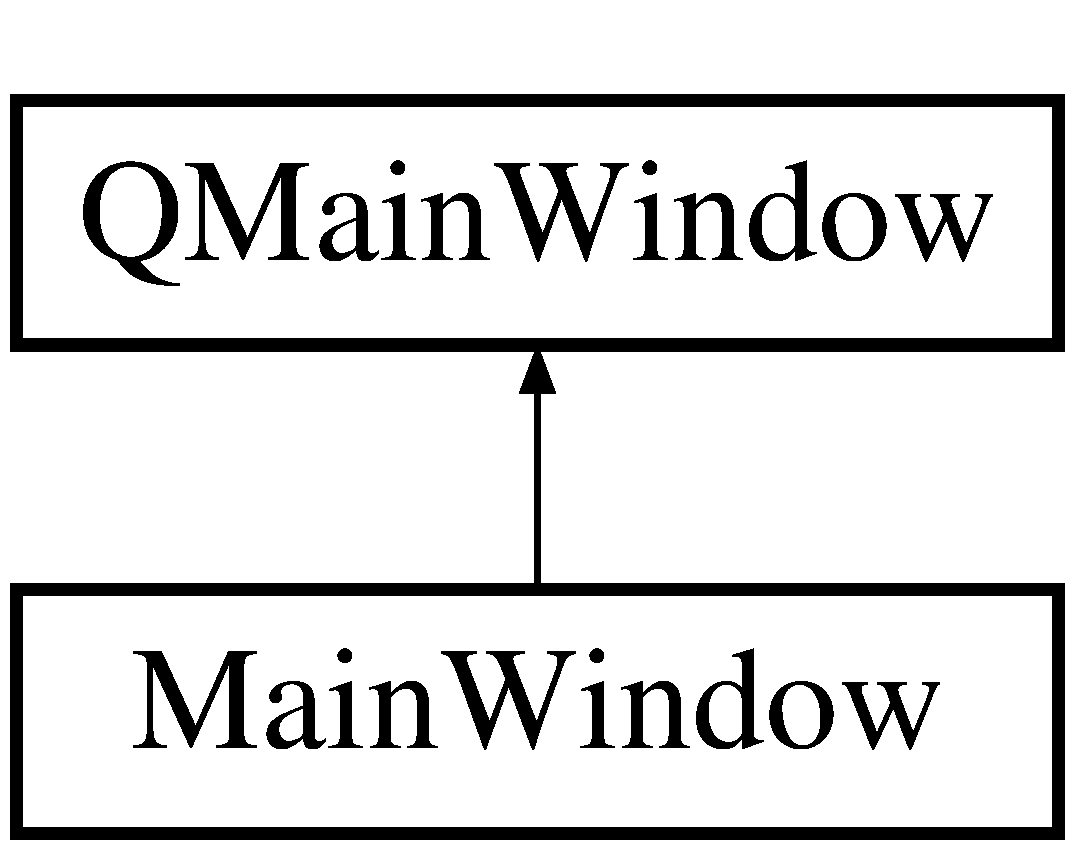
\includegraphics[height=2.000000cm]{class_main_window}
\end{center}
\end{figure}
\subsection*{Public Member Functions}
\begin{DoxyCompactItemize}
\item 
\hyperlink{class_main_window_a8b244be8b7b7db1b08de2a2acb9409db}{Main\-Window} (Q\-Widget $\ast$parent=0)
\item 
\hyperlink{class_main_window_ae98d00a93bc118200eeef9f9bba1dba7}{$\sim$\-Main\-Window} ()
\end{DoxyCompactItemize}
\subsection*{Private Slots}
\begin{DoxyCompactItemize}
\item 
void \hyperlink{class_main_window_a4de79c63c7fa0b8d7c468ac71f20be81}{on\-\_\-push\-Button\-\_\-clicked} ()
\begin{DoxyCompactList}\small\item\em \hyperlink{class_main_window_a4de79c63c7fa0b8d7c468ac71f20be81}{on\-\_\-push\-Button\-\_\-clicked()}; \end{DoxyCompactList}\item 
void \hyperlink{class_main_window_ae0e46dc3da4ee07bf66e73e20300220c}{on\-\_\-push\-Button\-\_\-2\-\_\-clicked} ()
\begin{DoxyCompactList}\small\item\em \hyperlink{class_main_window_ae0e46dc3da4ee07bf66e73e20300220c}{on\-\_\-push\-Button\-\_\-2\-\_\-clicked()}; \end{DoxyCompactList}\item 
void \hyperlink{class_main_window_a12cf88402a93adef89645ba4e4cb7be1}{on\-\_\-push\-Button\-\_\-3\-\_\-clicked} ()
\begin{DoxyCompactList}\small\item\em \hyperlink{class_main_window_a12cf88402a93adef89645ba4e4cb7be1}{on\-\_\-push\-Button\-\_\-3\-\_\-clicked()}; \end{DoxyCompactList}\end{DoxyCompactItemize}
\subsection*{Private Attributes}
\begin{DoxyCompactItemize}
\item 
Ui\-::\-Main\-Window $\ast$ \hyperlink{class_main_window_a35466a70ed47252a0191168126a352a5}{ui}
\end{DoxyCompactItemize}


\subsection{Detailed Description}
Main class of my application for project C\-S340. contains slots for three buttons they print \char`\"{}pushbutton\char`\"{}, \char`\"{}\-H\-E\-L\-L\-O\char`\"{}, and \char`\"{}\-W\-O\-R\-L\-D!\char`\"{} when clicked. 

Inherits for Q\-Main\-Window from Qt 

\subsection{Constructor \& Destructor Documentation}
\hypertarget{class_main_window_a8b244be8b7b7db1b08de2a2acb9409db}{\index{Main\-Window@{Main\-Window}!Main\-Window@{Main\-Window}}
\index{Main\-Window@{Main\-Window}!MainWindow@{Main\-Window}}
\subsubsection[{Main\-Window}]{\setlength{\rightskip}{0pt plus 5cm}Main\-Window\-::\-Main\-Window (
\begin{DoxyParamCaption}
\item[{Q\-Widget $\ast$}]{parent = {\ttfamily 0}}
\end{DoxyParamCaption}
)}}\label{class_main_window_a8b244be8b7b7db1b08de2a2acb9409db}
Constructor for \hyperlink{class_main_window}{Main\-Window}


\begin{DoxyParams}{Parameters}
{\em parent} & a parent widget, can be null \\
\hline
\end{DoxyParams}
\hypertarget{class_main_window_ae98d00a93bc118200eeef9f9bba1dba7}{\index{Main\-Window@{Main\-Window}!$\sim$\-Main\-Window@{$\sim$\-Main\-Window}}
\index{$\sim$\-Main\-Window@{$\sim$\-Main\-Window}!MainWindow@{Main\-Window}}
\subsubsection[{$\sim$\-Main\-Window}]{\setlength{\rightskip}{0pt plus 5cm}Main\-Window\-::$\sim$\-Main\-Window (
\begin{DoxyParamCaption}
{}
\end{DoxyParamCaption}
)}}\label{class_main_window_ae98d00a93bc118200eeef9f9bba1dba7}


\subsection{Member Function Documentation}
\hypertarget{class_main_window_ae0e46dc3da4ee07bf66e73e20300220c}{\index{Main\-Window@{Main\-Window}!on\-\_\-push\-Button\-\_\-2\-\_\-clicked@{on\-\_\-push\-Button\-\_\-2\-\_\-clicked}}
\index{on\-\_\-push\-Button\-\_\-2\-\_\-clicked@{on\-\_\-push\-Button\-\_\-2\-\_\-clicked}!MainWindow@{Main\-Window}}
\subsubsection[{on\-\_\-push\-Button\-\_\-2\-\_\-clicked}]{\setlength{\rightskip}{0pt plus 5cm}void Main\-Window\-::on\-\_\-push\-Button\-\_\-2\-\_\-clicked (
\begin{DoxyParamCaption}
{}
\end{DoxyParamCaption}
)\hspace{0.3cm}{\ttfamily [private]}, {\ttfamily [slot]}}}\label{class_main_window_ae0e46dc3da4ee07bf66e73e20300220c}


\hyperlink{class_main_window_ae0e46dc3da4ee07bf66e73e20300220c}{on\-\_\-push\-Button\-\_\-2\-\_\-clicked()}; 

prints \char`\"{}\-H\-E\-L\-L\-O\char`\"{} when clicked \hypertarget{class_main_window_a12cf88402a93adef89645ba4e4cb7be1}{\index{Main\-Window@{Main\-Window}!on\-\_\-push\-Button\-\_\-3\-\_\-clicked@{on\-\_\-push\-Button\-\_\-3\-\_\-clicked}}
\index{on\-\_\-push\-Button\-\_\-3\-\_\-clicked@{on\-\_\-push\-Button\-\_\-3\-\_\-clicked}!MainWindow@{Main\-Window}}
\subsubsection[{on\-\_\-push\-Button\-\_\-3\-\_\-clicked}]{\setlength{\rightskip}{0pt plus 5cm}void Main\-Window\-::on\-\_\-push\-Button\-\_\-3\-\_\-clicked (
\begin{DoxyParamCaption}
{}
\end{DoxyParamCaption}
)\hspace{0.3cm}{\ttfamily [private]}, {\ttfamily [slot]}}}\label{class_main_window_a12cf88402a93adef89645ba4e4cb7be1}


\hyperlink{class_main_window_a12cf88402a93adef89645ba4e4cb7be1}{on\-\_\-push\-Button\-\_\-3\-\_\-clicked()}; 

prints \char`\"{}\-W\-O\-R\-L\-D!\char`\"{} when clicked \hypertarget{class_main_window_a4de79c63c7fa0b8d7c468ac71f20be81}{\index{Main\-Window@{Main\-Window}!on\-\_\-push\-Button\-\_\-clicked@{on\-\_\-push\-Button\-\_\-clicked}}
\index{on\-\_\-push\-Button\-\_\-clicked@{on\-\_\-push\-Button\-\_\-clicked}!MainWindow@{Main\-Window}}
\subsubsection[{on\-\_\-push\-Button\-\_\-clicked}]{\setlength{\rightskip}{0pt plus 5cm}void Main\-Window\-::on\-\_\-push\-Button\-\_\-clicked (
\begin{DoxyParamCaption}
{}
\end{DoxyParamCaption}
)\hspace{0.3cm}{\ttfamily [private]}, {\ttfamily [slot]}}}\label{class_main_window_a4de79c63c7fa0b8d7c468ac71f20be81}


\hyperlink{class_main_window_a4de79c63c7fa0b8d7c468ac71f20be81}{on\-\_\-push\-Button\-\_\-clicked()}; 

prints \char`\"{}button\char`\"{} when clicked 

\subsection{Member Data Documentation}
\hypertarget{class_main_window_a35466a70ed47252a0191168126a352a5}{\index{Main\-Window@{Main\-Window}!ui@{ui}}
\index{ui@{ui}!MainWindow@{Main\-Window}}
\subsubsection[{ui}]{\setlength{\rightskip}{0pt plus 5cm}Ui\-::\-Main\-Window$\ast$ Main\-Window\-::ui\hspace{0.3cm}{\ttfamily [private]}}}\label{class_main_window_a35466a70ed47252a0191168126a352a5}


The documentation for this class was generated from the following files\-:\begin{DoxyCompactItemize}
\item 
\hyperlink{mainwindow_8h}{mainwindow.\-h}\item 
\hyperlink{mainwindow_8cpp}{mainwindow.\-cpp}\end{DoxyCompactItemize}

\chapter{File Documentation}
\hypertarget{main_8cpp}{\section{main.\-cpp File Reference}
\label{main_8cpp}\index{main.\-cpp@{main.\-cpp}}
}
{\ttfamily \#include \char`\"{}mainwindow.\-h\char`\"{}}\\*
{\ttfamily \#include $<$Q\-Application$>$}\\*
\subsection*{Functions}
\begin{DoxyCompactItemize}
\item 
int \hyperlink{main_8cpp_a0ddf1224851353fc92bfbff6f499fa97}{main} (int argc, char $\ast$argv\mbox{[}$\,$\mbox{]})
\end{DoxyCompactItemize}


\subsection{Function Documentation}
\hypertarget{main_8cpp_a0ddf1224851353fc92bfbff6f499fa97}{\index{main.\-cpp@{main.\-cpp}!main@{main}}
\index{main@{main}!main.cpp@{main.\-cpp}}
\subsubsection[{main}]{\setlength{\rightskip}{0pt plus 5cm}int main (
\begin{DoxyParamCaption}
\item[{int}]{argc, }
\item[{char $\ast$}]{argv\mbox{[}$\,$\mbox{]}}
\end{DoxyParamCaption}
)}}\label{main_8cpp_a0ddf1224851353fc92bfbff6f499fa97}

\hypertarget{mainwindow_8cpp}{\section{mainwindow.\-cpp File Reference}
\label{mainwindow_8cpp}\index{mainwindow.\-cpp@{mainwindow.\-cpp}}
}
{\ttfamily \#include $<$iostream$>$}\\*
{\ttfamily \#include \char`\"{}mainwindow.\-h\char`\"{}}\\*
{\ttfamily \#include \char`\"{}ui\-\_\-mainwindow.\-h\char`\"{}}\\*

\hypertarget{mainwindow_8h}{\section{mainwindow.\-h File Reference}
\label{mainwindow_8h}\index{mainwindow.\-h@{mainwindow.\-h}}
}
{\ttfamily \#include $<$Q\-Main\-Window$>$}\\*
\subsection*{Classes}
\begin{DoxyCompactItemize}
\item 
class \hyperlink{class_main_window}{Main\-Window}
\begin{DoxyCompactList}\small\item\em Main class of my application for project C\-S340. contains slots for three buttons they print \char`\"{}pushbutton\char`\"{}, \char`\"{}\-H\-E\-L\-L\-O\char`\"{}, and \char`\"{}\-W\-O\-R\-L\-D!\char`\"{} when clicked. \end{DoxyCompactList}\end{DoxyCompactItemize}


\subsection{Detailed Description}
\begin{DoxyAuthor}{Author}
Luc Renambot 
\end{DoxyAuthor}
\begin{DoxyVersion}{Version}
1.\-0 
\end{DoxyVersion}
\hypertarget{mainwindow_8h_LICENSE}{}\subsection{L\-I\-C\-E\-N\-S\-E}\label{mainwindow_8h_LICENSE}
blah blah \hypertarget{mainwindow_8h_DESCRIPTION}{}\subsection{D\-E\-S\-C\-R\-I\-P\-T\-I\-O\-N}\label{mainwindow_8h_DESCRIPTION}
blah blah blah 
%--- End generated contents ---

% Index
\newpage
\phantomsection
\addcontentsline{toc}{part}{Index}
\printindex

\end{document}
